\section{换热式固定床反应器}


\begin{frame}
    \frametitle{换热式固定床反应器}

        \begin{minipage}{0.65\linewidth}
            \begin{itemize}
                \item 换热式固定床反应器，又称非绝热变温反应器
                \item 催化剂可以放在管内，也可放在管间
                \item 大多数是采用自上而下的流动方式
                \item 载热体在管间流动，流向可以与反应气体成逆流，也可以成并流
                \item 换热强度应满足反应过程所要求的温度条件
            \end{itemize}
        \end{minipage}\hfill
        \begin{minipage}{0.32\linewidth}
            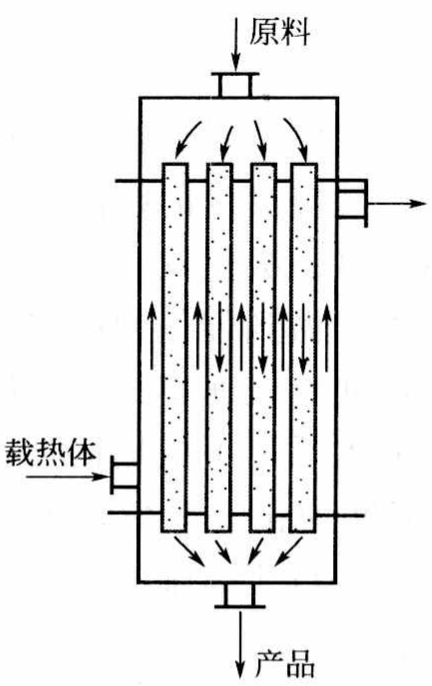
\includegraphics[width=.95\linewidth]{figures/fig7.5.png}
        \end{minipage}

\end{frame}


\begin{frame}
    \frametitle{换热式固定床反应器}

    对于换热式列管反应器，载热体的合理选择，往往是控制反应温度和保持反应器操作条件稳定的关键。载热体的温度与床层
反应温度之间的温度差宜小，但又必须能将反应放出的热量带走。这就要求在传热面积一定的情况下，有较大的传热系数。
    \begin{itemize}
        \item 473K，加压热水
        \item 523 $\sim$ 573K，挥发性低的有机物
        \item 573K以上，无机熔盐
        \item 873K以上，烟道气
    \end{itemize}

\end{frame}


\begin{frame}
    \frametitle{换热式固定床反应器}

    换热式固定床反应器的特点：
    \begin{itemize}
        \item 反应管直径一般都比较小，多为20 $\sim$ 35mm。
        \item 列管可多达20000根
        \item 可用于放热反应，也可用于吸热反应，后者更为常见。
        \item 床层轴向温度分布相对来说比较均匀
        \item 催化剂磨损小、返混小和催化剂生产能力较高
        \item 反应器便于放大
        \item[\times] 结构比绝热反应器复杂
        \item[\times] 催化剂的装卸不方便
    \end{itemize}

\end{frame}


\begin{frame}
    \frametitle{进行单一反应时的分析}

    换热式固定床反应器中温度与转化率的关系式如下：
    \[
        \frac{\mathrm{d} T}{\mathrm{~d} X_{\mathrm{A}}}=\frac{w_{\mathrm{A} 0}(-\Delta H_{\mathrm{r}})}{M_{\mathrm{A}} C_{p \mathrm{t}}}-\frac{4 U w_{\mathrm{A} 0}(T-T_{\mathrm{C}})}{d_{\mathrm{t}} M_{\mathrm{A}} C_{p \mathrm{t}} \eta_{0} \rho_{\mathrm{b}}(-\mathscr{R}_{\mathrm{A}})}
    \]
    若以$\bar{C}_{p \mathrm{t}}$代替$C_{p \mathrm{t}}$，
    \[
        \frac{\mathrm{d} T}{\mathrm{d} X_{\mathrm{A}}}=\lambda-\frac{4 U w_{\mathrm{A} 0}(T-T_{\mathrm{C}})}{d_{\mathrm{t}} M_{\mathrm{A}} \bar{C}_{p \mathrm{t}} \eta_{0} \rho_{\mathrm{b}}(-\mathscr{R}_{\mathrm{A}})}
    \]
    \begin{itemize}
        \item 可逆吸热反应和不可逆的吸热或放热反应，维持在尽可能高的温度下操作是有利的，因之力图做到催化剂床层温度均匀最可取。
        \item 可逆放热反应，应使转化率与温度的关系尽可能地接近最佳温度曲线。
    \end{itemize}

\end{frame}


\begin{frame}
    \frametitle{换热式固定床反应器的$T-X_\mathrm{A}$图}

    \begin{figure}[htpb]
        \centering
        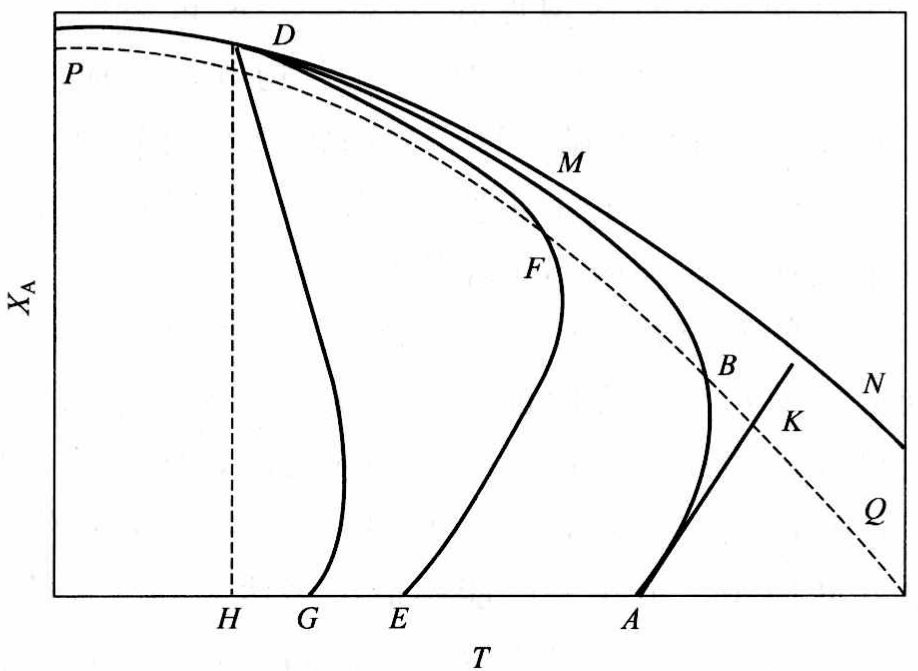
\includegraphics[width=.63\linewidth]{figures/fig7.6.png}
    \end{figure}

\end{frame}


\begin{frame}
    \frametitle{热点温度}
    \begin{enumerate}
      \item 反应初期远离平衡 ， 反应速率大 ， 以致反应放热速率大于冷却介质移热速率 ， 因而温度随转化率的增加而升高 。
      \item 反应后期则相反 ， 移热速率大于放热速率 ， 温度随转化率的增加而降低 。
      \item 在极大值处 ， $\dif T/\dif X_\mathrm{A}=0$ ，$\dif T/\dif Z=0$  。 这一最高温度称为\highlight{热点温度} 。
      \item 在实际生产中 ， 热点的位置及其温度的高低是反应器操作控制的一个极为重要的依据 ， 借此可判断反应器运转的情况 。 
      \item 只要热点温度不超过允许温度 ， 床层的其他部位也绝不会超过 。
    \end{enumerate}
       
\end{frame}


\begin{frame}
    \frametitle{反应的评价}
    \begin{enumerate}
      \item 比较这几条曲线可知 ， 它们接近最佳温度曲线的程度是不同的 ， 差别的存在是进料温度不同的结果 。
      \item 进料温度太高或过低都会偏离最佳温度曲线太远 ， 因之存在一最佳进料温度 。
      \item 无论哪一条曲线在反应初期都偏离最佳温度曲线甚远 ， 但这对整个反应过程来说 ， 并不会产生很大的影响 。 反应初期的反应速率要远大于反应后期 ， 因而反应温度偏离最佳值所带来的影响远小于中后期 。
      \item 所以 ， 评价 $T-X_\mathrm{A}$ 曲线的优劣主要是看反应中后期接近最佳温度曲线的程度 。
      \item 曲线 EFD 较曲线 ABD 要好 。
    \end{enumerate}
\end{frame}


\begin{frame}
    \frametitle{进行复合反应时的分析}

    在换热式固定床反应器内进行复合反应时，由于副反应的存在而使问题变得复杂。

    以钒催化剂上邻二甲苯氧化反应为例，略去次要反应，整个反应过程简化如下：

    \begin{minipage}{0.48\linewidth}
        \begin{center}
            \begin{tikzpicture}[scale=0.9]
                \node (A) at (135:4) {邻二甲苯(A)};
                \node (B) at (45:4) {苯酐(B)};
                \node (C) at (0,0) {8(\ch{CO2,CO})(C)};
                % \draw (A) -- (B) -- (C) -- (A);
                \draw[->] (A) -- (B) node[above,midway]{$k_1$};
                \draw[->] (A) -- (C) node[above,midway]{$k_3$};
                \draw[->] (B) -- (C) node[above,midway]{$k_2$};
                \end{tikzpicture}
            \end{center}
    \end{minipage}\hfill
    \begin{minipage}{0.48\linewidth}
        \[
            \begin{aligned}
                \overline{r_1}=&k_1p_\text{A}p_0,\quad k_1=0.04017\exp\left(-\frac{13500}{T}\right)\\
                \overline{r_2}=&k_2p_\text{B}p_0,\quad k_2=0.1175\exp\left(-\frac{15500}{T}\right)\\
                \overline{r_3}=&k_3p_\text{A}p_0,\quad k_3=0.01688\exp\left(-\frac{14300}{T}\right)
            \end{aligned}
        \]
    \end{minipage}
    
    所考察的三个反应只有两个是独立的。建立反应器的数学模型时，需有两个物料衡算式和一个热量衡算式。

\end{frame}


\begin{frame}
    \frametitle{建立数学模型}
    采用拟均相模型 ， 选择苯酐的收率$Y_\mathrm{B}$、 一氧化碳和二氧化碳的总收率$Y_\mathrm{C}$ 以及温度 $T$ 为状态变量 ， 轴向距离 $Z$ 为控制变量 ， 数学模型方程如下
    $$\begin{gathered}
        \frac{Gy_{\mathrm{A}0}}{M_{\mathrm{m}}}\frac{\mathrm{d}Y_{\mathrm{B}}}{\mathrm{d}Z}=\rho_{\mathrm{b}}\mathscr{R}_{\mathrm{B}} \\
        8\frac{Gy_{\mathrm{A}0}}{M_{\mathrm{m}}}\frac{\mathrm{d}Y_{\mathrm{C}}}{\mathrm{d}Z}=\rho_{\mathrm{b}}{\mathscr{R}}_{\mathrm{C}} \\
        GC_{pt}{\frac{\mathrm{d}T}{\mathrm{d}Z}}=\rho_{\mathrm{b}}\mathscr{R}_{\mathrm{B}}(-\Delta H_{r})_{\mathrm{B}}+\rho_{\mathrm{b}}\mathscr{R}_{\mathrm{C}}(-\Delta H_{r})_{\mathrm{C}}-{\frac{4U}{d_{t}}}(T-T_{c}) 
    \end{gathered}$$
\end{frame}


\begin{frame}
    \frametitle{对邻二甲苯催化氧化反应器进行模拟}
    现选定进反应器的原料气中邻二甲苯的摩尔分数为 0.8432\%， 氧为 20.33\%；
    
    混合气的平均相对分子质量$M_\mathrm{m}=29.29$；
    
    反应管内径 $d_\mathrm{t}=26$mm；
    
    操作压力$p=$ \num{1.274e5}Pa；
    
    管外用熔盐冷却并作强制循环，熔盐温度恒定且与进入床层的原料气温度相等，$T_\mathrm{C} = T_0$；
    
    床层与熔盐间的总传热系数 $U=$ \SI{508}{kJ/(m^2.h.K)}；
    
    床层内气体的质量速度$G=$ \SI{2.984}{kg/(m^2.s)}；
    
    床层的堆密度 $\rho_{\mathrm{b}}= 1300$ \si{kg/m^3}；
    
    热力学数据：$C_{pt}= 1. 059$\si{kJ/(kg.K)}，$(-\Delta H_{r})_{\mathrm{B}}=1285$ kJ/mol， $(-\Delta H_{r})_{\mathrm{C}}=4561$kJ/mol。 
\end{frame}


\begin{frame}
    \frametitle{模型求解}
    将数据代入模型方程，化简后得
    \[
        \begin{aligned}
                \frac{\mathrm{d}Y_{\mathrm{B}}}{\mathrm{d}Z}=&4.748\times10^{8}\bigg[(1-Y_{\mathrm{B}}-Y_{\mathrm{C}})\exp\bigg(-\frac{135000}{T}\bigg)-2.781Y_{\mathrm{B}}\exp\bigg(-\frac{155000}{T}\bigg)\bigg]  \\
                \frac{\mathrm{d}Y_{\mathrm{c}}}{\mathrm{d}Z}=&1.995\times10^{8}\Big[(1-Y_{\mathrm{B}}-Y_{\mathrm{C}})\exp\Big(-\frac{14300}{T}\Big)+6.621Y_{\mathrm{B}}\exp\Big(-\frac{155000}{T}\Big)\Big]  \\
                \frac{\mathrm{d}T}{\mathrm{d}Z}=&1.661\times10^{11}\Big[(1-Y_{\mathrm{B}}-Y_{\mathrm{C}})\exp\Big(-\frac{135000}{T}\Big)-2.781Y_{\mathrm{B}}\exp\Big(-\frac{15500}{T}\Big)\Big]+  \\
                &2.477\times10^{11}\Big[(1-Y_{\mathrm{B}}-Y_{\mathrm{C}})\exp\Big(-\frac{14300}{T}\Big)+6.619Y_{\mathrm{B}}\exp\Big(-\frac{15500}{T}\Big)\Big]- \\
                &7.232(T-T_{\mathrm{C}})
        \end{aligned}
    \]
    初值条件：$Z=0, Y_\mathrm{B}=0, Y_\mathrm{C}=0, T=T_0=T_\mathrm{C}$。

    现对不同的进料温度，用龙格-库塔法进行求解。
\end{frame}


\begin{frame}
    \frametitle{邻二甲苯氧化反应器床层的轴向温度分布}

        \begin{minipage}{0.39\linewidth}
            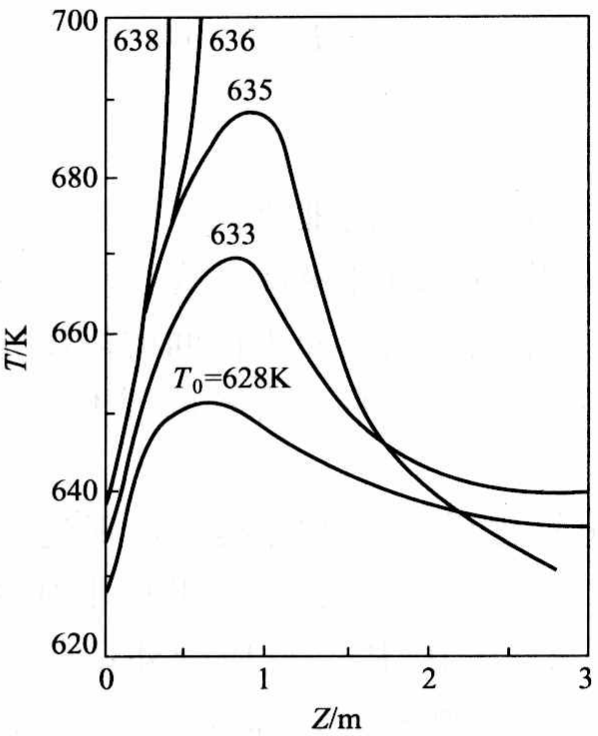
\includegraphics[width=\linewidth]{figures/fig7.7.png}
        \end{minipage}\hfill
        \begin{minipage}{0.58\linewidth}
            \begin{itemize}
                \item 当$T_0=628 \sim 635$K时，轴向温度分布曲线都存在极大值，即热点。
                \item 热点温度与进料温度相差达数十度
                \item 进料温度越高，相差越大，热点位置越向后移。
                \item 进料温度为636 K时，其热点温度已升得十分高，以致反应器操作遭到破坏。
                \item 进料温度1度之差竟造成如此严重的后果，这种现象称为\highlight{飞温}。
            \end{itemize}
        \end{minipage}

\end{frame}


\begin{frame}
    \frametitle{邻二甲苯氧化反应器的苯酐收率的轴向分布}

        \begin{minipage}{0.42\linewidth}
            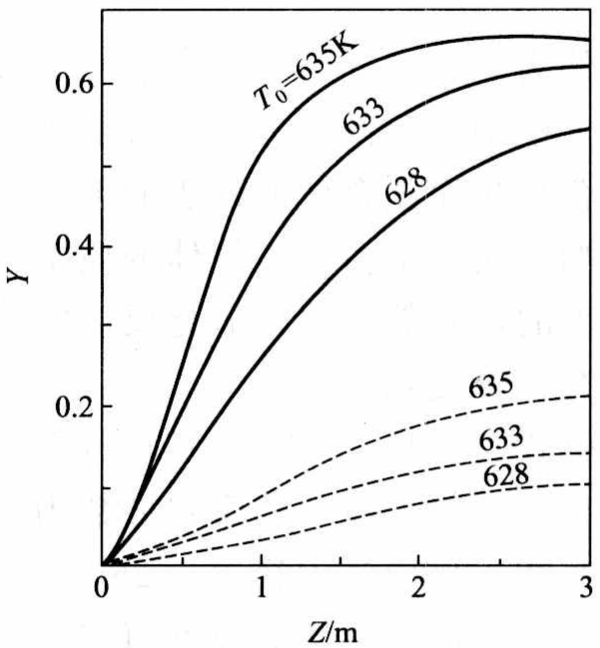
\includegraphics[width=\linewidth]{figures/fig7.8.png}
        \end{minipage}\hfill
        \begin{minipage}{0.56\linewidth}
            \begin{itemize}
                \item 实曲线为苯酐收率$Y_\mathrm{B}$
                \item 虚曲线为\ch{CO2,CO}收率$Y_\mathrm{C}$
                \item $Y_\mathrm{B}$，$Y_\mathrm{C}$均随床层高度的增加而增加
                \item 当进料温度提高时，只要不出现飞温，$Y_\mathrm{B}$，$Y_\mathrm{C}$也都增加。
                \item 628K时选择性为83.4\%，633K时选择性为80.5\%，反应选择性随进料温度的增加而降低。
                \item 进料温度的选择必须兼顾收率与反应选择性这两个方面。
            \end{itemize}
        \end{minipage}

\end{frame}